\documentclass{beamer}

\usepackage{beamerthemesplit} % new
\usepackage[utf8]{inputenc}
\usepackage[spanish,activeacute]{babel}
\usepackage{graphicx}
\graphicspath { {media/} }
\newcommand\floor[1]{\lfloor#1\rfloor}
\newcommand{\Mod}[1]{\ (\mathrm{mod}\ #1)}

%\hypersetup{pdfpagemode=FullScreen}
\begin{document}
\title{AS combinadas \\ Intercambio de llaves \\ Suites criptográficas}   
\author{González Vargas \\ Acosta Hernández} 
\date{Criptografía y seguridad 2017-2 \\ Facultad de Ciencias UNAM} 

\frame{\titlepage} 
\frame[allowframebreaks]{\frametitle{Contenido}\tableofcontents} 


\section{Combinación de Asociaciones de Seguridad}
\subsection{Preliminares}
\frame{\frametitle{Recordando...}
  \begin{itemize}
  \item Asociaciones de seguridad 
  \item Modos de uso en SA
  \end{itemize}
}
\subsubsection{Asociaciones de seguridad}
\frame{\frametitle{Definición}
  Es una conexión lógica de un sólo sentido entre un emisor
  y un receptor que proporciona servicios de seguridad al tráfico de información
  que se transporta en ella.
}

\subsubsection{Modos de uso en SA}
\frame{\frametitle{Modo de transporte}
  \begin{itemize}
  \item Utilizado para cifrar y opcionalmente autentificar los datos de IP.
  \item Adecuado para proteger conexiones entre \textit{hosts}, que soportan \textit{ESP}.\\

    Ventaja: Provee confidencialidad para cualquier aplicación que la utilice.\\
    Desventaja: Es susceptible a análisis de tráfico.
  \end{itemize}
}

\frame{\frametitle{Modo túnel}
  \begin{itemize}
  \item Es utilizado para cifrar un paquete IP por completo.
  \item Orientado para sistemas que incluyen un \textit{firewall}, o algún otro
    mecanismo de seguridad que protege una red confiable de redes externas.
    Ventaja: Resistente a análisis de tráfico.
  \end{itemize}
}

\subsection{Combinación de SAs}
\frame{\frametitle{¿Para qué?}
  Una asociación de seguridad puede implementar ya sea un protocolo \textit{AH}
  o un \textit{ESP}, pero sólo uno.
  Sin embargo, puede ocurrir que un flujo de tráfico llame servicios de ambos protocolos
  durante su operación. En otro caso, puede que dicho flujo necesite de los servicios de \textit{IPsec} entre \textit{hosts} y, para ese mismo flujo, servicios separados entre \textit{gateways}.
  Múltiples SAs, deben ser utilizados para obtener los servicios de \textit{IPsec}.
}

\frame{\frametitle{Colecciones de SAs}
  Secuencia de \textbf{SA}s a través de las cuáles el tráfico de datos debe ser procesado
  para obtener los servicios de \textit{IPsec} que se necesitan.
  Se puede obtener una combinación de SAs mediante:
  \begin{itemize}
  \item Transport Adjacency
  \item Iterated Tunneling
  \end{itemize}
}

\frame{\frametitle{Transport Adjacency}
  Consiste en aplicar más de un protocolo de seguridad a un mismo paquete \textit{IP} sin invocar
  un modo túnel. Se realiza sólo un nivel de anidamiento, pues el procesamiento es realzado
  para una única instancia de \textit{IPsec}, el punto de destino del paquete.
}
\frame{\frametitle{Iterated Tunneling}
  Consiste en aplciar múltiples capas de protocolos de seguridad a un paquete, efectuadas a través de tunelizado de \textit{IP}.
  Este enfoque permite varios niveles de anidamiento dado que cada túnel puede originarse o terminar en un punto
  de \textit{IPsec} a lo largo de la trayectoria del paquete.
}

\frame{\frametitle{Combinación}
  Ambos enfoques pueden ser combinados al hacer que, por ejemplo, una \textbf{SA} de transporte entre \textit{hosts} viaje parte del camino por medio de un \textbf{SA} de túnel entre \textit{gateways} de
  seguridad.
  Un interrogante potencial al tener colecciones de \textbf{SA}s, es el orden en que la autenticación y el cifrado deben ser aplicados entre dos puntos de destino y las maneras para conseguir el apropiado.  
}

%i y ii
\subsection{Autenticación y confidencialidad}
\frame{\frametitle{Autenticación y confidencialidad}
  Siempre que la comunicación entre \textit{hosts} requiera tanto de un cifrado como una autenticación, ambos pueden combinarse y aplicarse en la transmisión de paquetes \textit{IP}. 
}

\subsubsection{Diferentes opciones}
\frame{\frametitle{ESP con Autenticación}
  El usuario apica primero \textit{ESP} a la información que debe ser protegida y posteriormente agrega al final el campo de autenticación.  \\
  \vspace{0.3cm}
  Se tienen dos casos:\\
}

\frame{\frametitle{ESP con Autenticación}
  \begin{itemize}
  \item \textbf{Transport Mode ESP}
     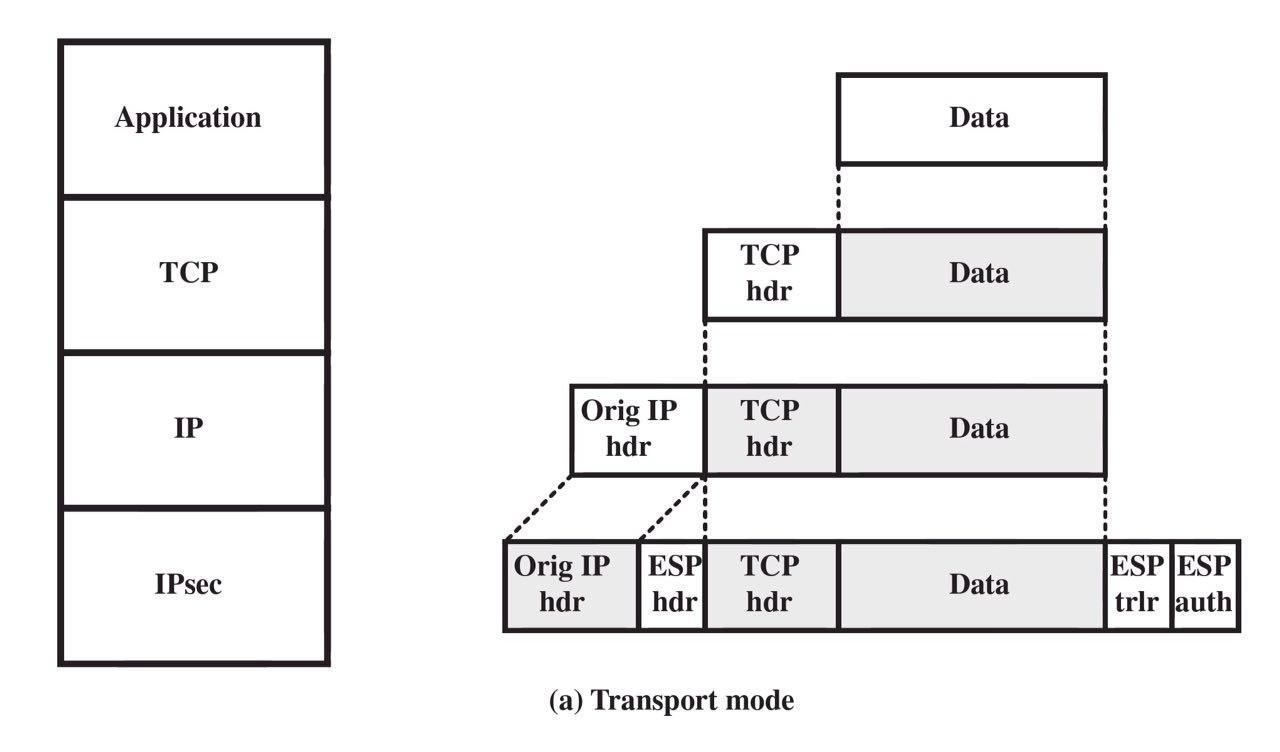
\includegraphics[scale=0.20]{ESPauthTrans.jpg}
    %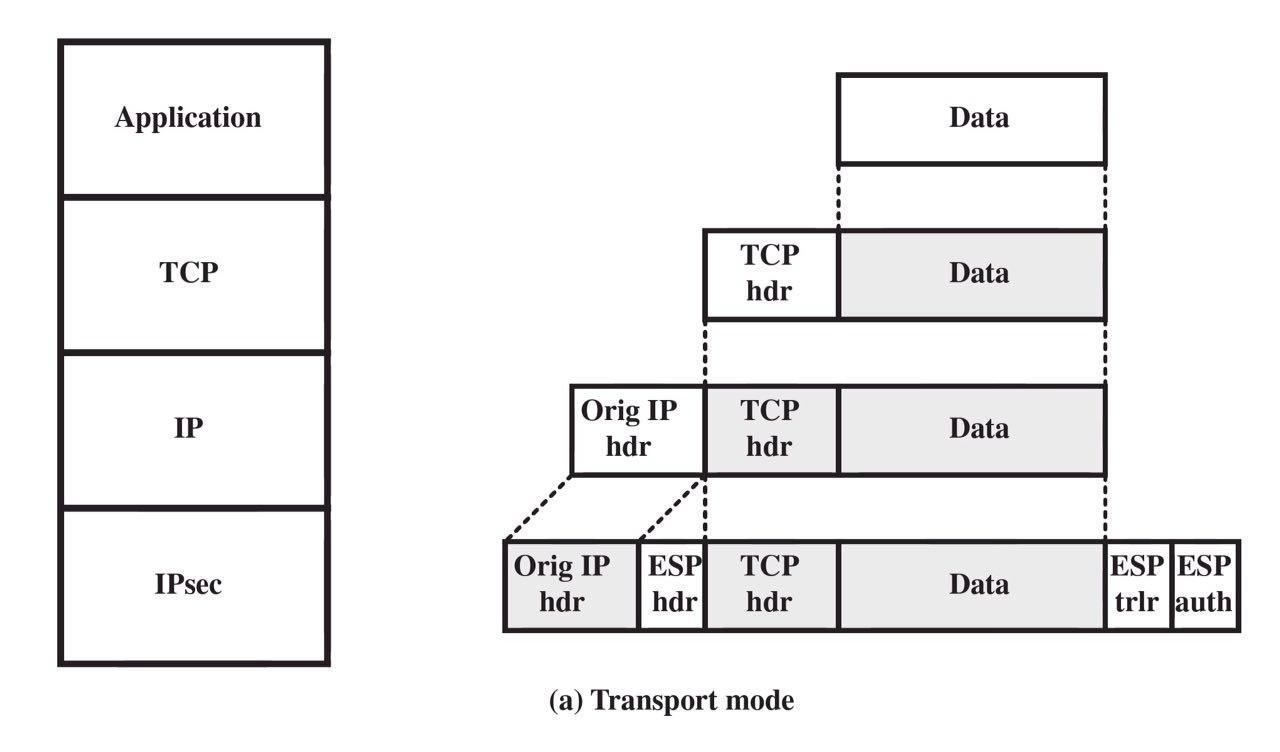
\includegraphics[width=1\textwidth]{ESPauthTrans}
  \end{itemize}
}

\frame{\frametitle{ESP con Autenticación}
  \begin{itemize}
  \item \textbf{Tunnel Mode ESP}
    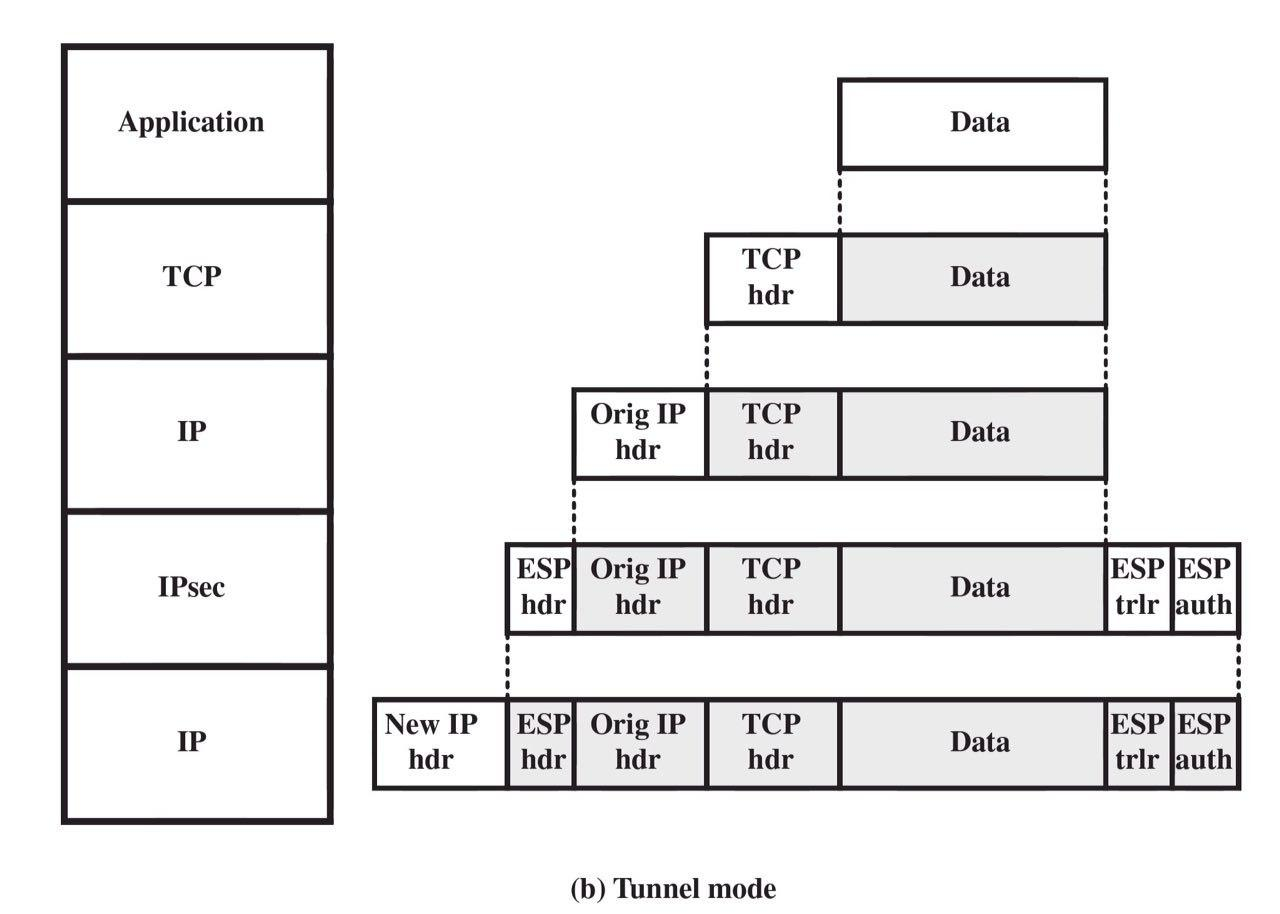
\includegraphics[scale=0.20]{ESPauthTun.jpg}
  \end{itemize}
}
  

\frame{\frametitle{Transport Adjacency}
  Se utilizan dos \textit{SAs} de transporte agrupadas, la primera o interior
  consta de aplicar \textit{ESP} sin autenticación, la segunda o exterior, consta de aplicar \textit{AH}
  en modo de transporte para que pueda cubrir tanto la parte del \textit{ESP} y la cabecera original del paquete.
}

\frame{\frametitle{Transport-Tunnel Bundle}
  En este caso se utiliza primero autenticación y posteriormente cifrado.
  Se aplica la asociación de seguridad \textit{AH} sobre la carga útil del paquete \textit{IP} junto con su cabecera. El paquete resultante
  se procesa con una segunda asociación de seguridad \textit{ESP} con modo de túnel. Al ser aplicado sobre todo el paquete, debe agregarse
  una nueva cabecera \textit{IP}.
}


\subsection{Combinaciones básicas}
\frame{\frametitle{Combinaciones básicas de SAs}
  \textbf{Caso 1.}
  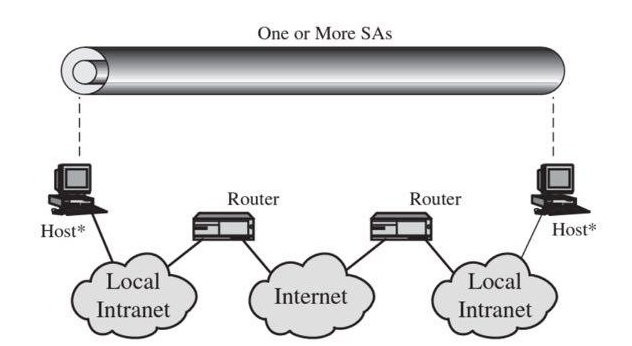
\includegraphics[scale=0.45]{caso1}
}

\frame{\frametitle{Combinaciones básicas de SAs}
  \textbf{Caso 2.}
  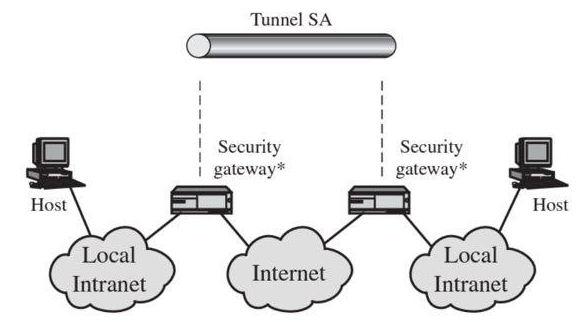
\includegraphics[scale=0.47]{caso2}
}

\frame{\frametitle{Combinaciones básicas de SAs}
  \textbf{Caso 3.}
  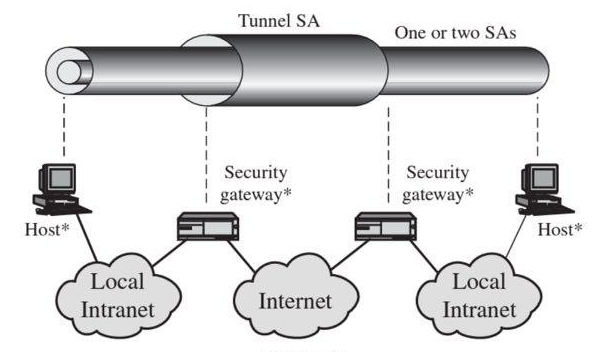
\includegraphics[scale=0.45]{caso3}
}

\frame{\frametitle{Combinaciones básicas de SAs}
  \textbf{Caso 4.}\\
  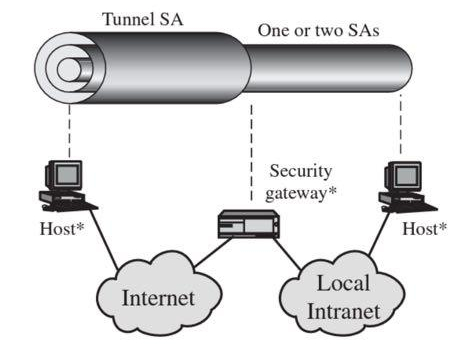
\includegraphics[scale=0.45]{caso4}
}


\section{Internet Key Exchange (IKE)} 
\subsection{Definición}
\frame{\frametitle{Internet Key Exchange (IKE)}
  Determinación y distribución de llaves secretas. Típicamente se requiere de cuatro llaves, dos pares para transmisión y recepción (para integridad y confidencialidad). \\~\\

  Tipos de manejo de llaves:
  \begin{itemize}
  \item \textbf{Manual:} Un administrador configura cada sistema con sus propias llaves y las de otros sistemas.
  \item \textbf{Automatizado:} Un sistema automatizado permite la creación de llaves para las asociaciones de seguridad.
  \end{itemize}
}

\frame{\frametitle{ISAKMP/Oakley}
  Protocolo por defecto de manejamiento de llaves automatizado. Consiste en: \\
  \begin{itemize}
  \item \textbf{Protocolo de determinación de llaves Oakley}: Protocolo de intercambio de llaves basado en el algoritmo Diffie-Hellman con seguridad agregada.
  \item \textbf{Asociación de seguridad de Internet y Protocolo de Manejo de Llaves (ISAKMP)}: ISAKMP provee un framework para el manejo de llaves por internet.
  \end{itemize}  
}

\subsection{Protocolo de determinación de llaves}
\frame{\frametitle{Protocolo de determinación de llaves}
  Refinamiento del intercambio de llaves Diffie-Hellman: \\~\\
  
  A y B se ponen de acuerdo en $q$ y $\alpha$ (raíz primitiva). \\  
  A selecciona $X_A$, B selecciona $X_B$ \\
  A calcula $Y_A \equiv \alpha^{X_A} \Mod{q}$, B calcula $Y_B \equiv \alpha^{X_B} \Mod{q}$ \\
  A y B calculan la llave secreta $K$: \\
  $K \equiv (Y_B)^{X_A} \Mod{q} \equiv (Y_A)^{X_B} \Mod{q} \equiv \alpha^{X_AX_B} \Mod q$
}

\frame{\frametitle{Protocolo de determinación de llaves}
  Beneficios de Diffie-Hellman: \\~\\
  
  \begin{itemize}
  \item Las llaves se crean cuando se necesitan.
  \item Sólo de necesita ponerse de acuerdo en los parámetros globales.
  \end{itemize}  
}

\frame{\frametitle{Protocolo de determinación de llaves}
  Debilidades de Diffie-Hellman: \\~\\
  
  \begin{itemize}
  \item No provee información sobre los participantes.
  \item Susceptible al ataque $man$-$in$-$the$-$middle$.
  \item Es intenso computacionalmente, lo que lo hace vulnerable a ataques de $clogging$.
  \end{itemize}
}

\subsubsection{Propiedades de IKE}

\frame{\frametitle{Propiedades de IKE}
  \begin{itemize}
  \item Utiliza cookies para evitar ataques de $clogging$.
  \item Permite negociar los parámetros globales.
  \item Utiliza $nonces$ para evitar ataques de repetición.
  \item Permite que se lleve acabo el intercambio de llaves públicas de Diffie-Helman.
  \item Autentifica para evitar ataques $man$-$in$-$the$-$middle$.
  \end{itemize}
}

\frame{\frametitle{Cookies}
  \textbf{Problema}: Oponente se hace pasar por una fuente legítima y manda repetidamente llaves públicad de Diffie-Hellman a la víctima. \\~\\

  \textbf{Solución}: Intercambio de $cookies$. Cada lado manda un número aleatorio ($cookie$) que es reconocido por el otro lado. Este reconocimiento se repite en el primer mensaje del intercabio Diffie-Hellman.
}

\frame{\frametitle{Cookies}
  Carácterísticas del cookie: \\~\\

  \begin{itemize}
  \item Depende de los lados que se comunican.
  \item No debe ser posible, más que para la entidad que le concierne, generar cookies que serán aceptadas por dicha entidad. Se usa información local secreta en el uso y verificación del cookie.
  \item La generación y verificación de cookies debe ser rápida.
  \end{itemize}
}

\frame{\frametitle{Grupos para D-H}
  Exponenciación modular con módulo de 768 bits \\
  $q = 2^{768} - 2^{704} - 1 + 2^{64} \times (\floor{2^{638} \times \pi} + 149686)$ \\
  $\alpha = 2$ \\~\\

  Exponenciación modular con módulo de 1024 bits \\
  $q = 2^{1024} - 2^{960} - 1 + 2^{64} \times (\floor{2^{864} \times \pi} + 129093)$ \\
  $\alpha = 2$ \\~\\

  Exponenciación modular con módulo de 1536 bits.
  
}

\frame{\frametitle{Grupos para D-H}
  Curva elíptica sobre $2^{155}$ \\
  Generador: (7B, 1C8) \\
  Parámetros: A = 0, B = 1EE9 \\~\\

  Curva elíptica sobre $2^{185}$ \\
  Generador: (18, D) \\
  Parámetros: A = 0, B = 1EE9
}

\frame{\frametitle{Métodos de Autenticación}
  \begin{itemize}
  \item \textbf{Firmas digitales}: Se firma un hash por ambos lados, cada uno con su propia llave privada. El hash se genera con el ID de usuario y $nonces$.
  \item \textbf{Cifrado de llave publica}: Se cifran parámetros como IDs y $nonces$ con la llave privada del remitente.
  \item \textbf{Cifrado de llave simétrica}: Se usa un sistema de cifrado simétrico.
  \end{itemize} 
}

\subsubsection{IKEv2}
\frame{\frametitle{IKEv2}
  Se intercambian mensajes en pares. Los primeros pares son los \textsf{intercambios iniciales}. \\~\\
  \begin{itemize}
  \item \textbf{Primer intercambio}: Se intercambia información sobre los algoritmos criptográficos y otros parámetros de seguridad a usar, a demás de $nonces$ y valores para Diffie-Hellman. Se crea IKE SA.
  \item \textbf{Segundo intercambio}: Los lados se autentican entre sí, se crea la primer SA de IPsec para proteger la comunicación ordinaria (se establece la SA de uso general).
  \end{itemize}
}

\subsection{Formatos de encabezado y de carga útil}

\subsubsection{Formato del encabezado IKE}
\frame{\frametitle{Formato del encabezado de IKE}
  IKE define procedimientos y formatos de paquete para establecer, negociar, modificar y eliminar asociaciones de seguridad. \\~\\
  Un mensaje IKE consiste de un encabezado IKE seguido de una o más cargas útiles. Se manejan con el protocolo de transporte.
}

\frame{\frametitle{Formato del encabezado de IKE}
  \begin{center}
    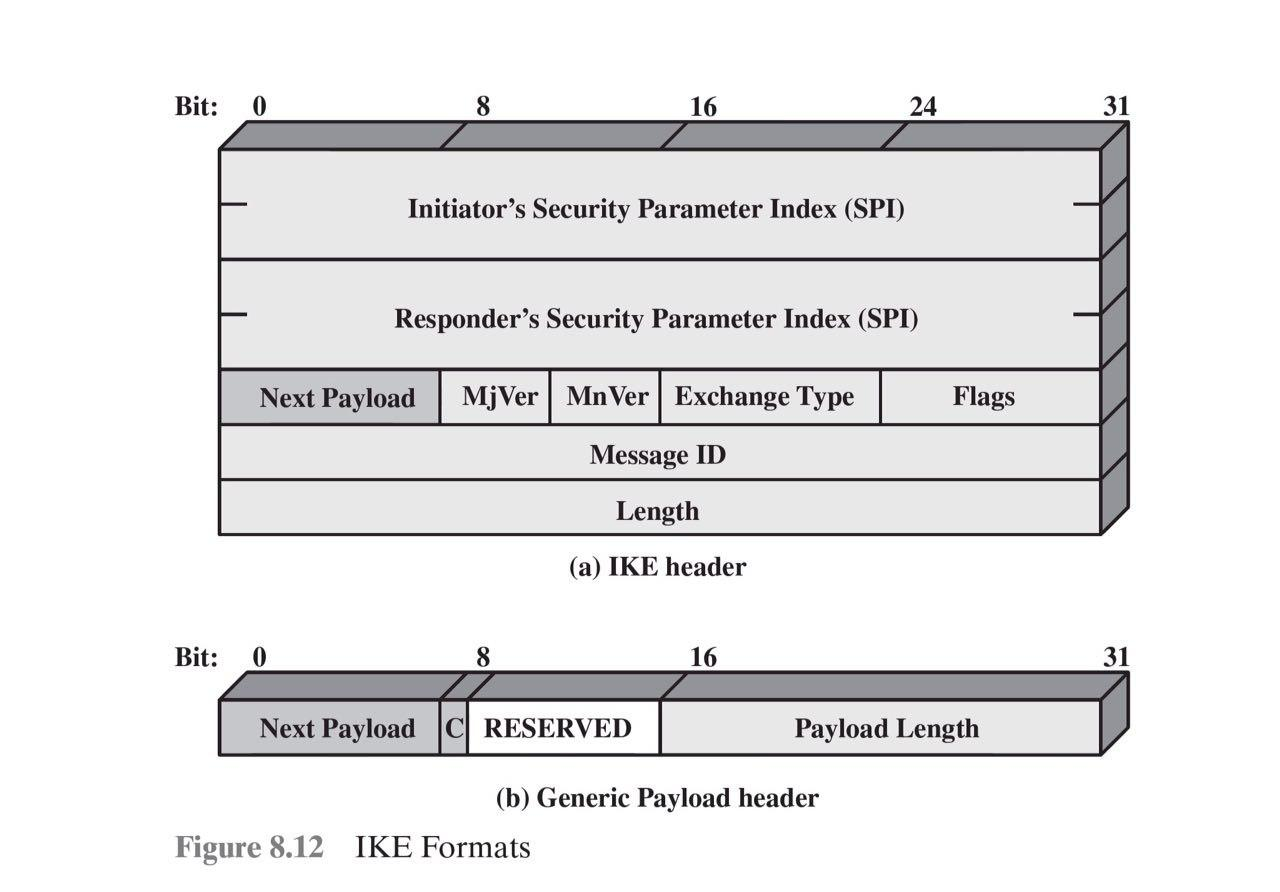
\includegraphics[scale=0.20]{IKEheader.jpg}
  \end{center}
}

\frame{\frametitle{Formato del encabezado de IKE}
  \begin{itemize}
  \item \textbf{Initiator SPI (64 bits)}: Valor escogido por el iniciador para identificar a una SA de IKE única.
  \item \textbf{Responder SPI (64 bits)}: Valor escogido por el recibidor par aidentificar a una SA de IKE única.
  \item \textbf{Next Payload (8 bits)}: Tipo de la primera carga útil en el mensaje.
  \item \textbf{Major Version (4 bits)}: Versión mayor de IKE en uso.
  \item \textbf{Minor Version (4 bits)}: Versión menor de IKE en uso.
  \end{itemize}
}

\frame{\frametitle{Formato del encabezado de IKE}
  \begin{itemize}
  \item \textbf{Exchange Type (8 bits)}: Tipo de intercambio.
  \item \textbf{Flags (8 bits)}: Opciones específicas dispuestas para el intercambio IKE.
  \item \textbf{Message ID (32 bits)}: Se usa para controlar retransmisión de paquetes perdidos y para corresponder solicitudes y respuestas.
  \item \textbf{Length (32 bits)}: Longitud total del mensaje en octetos.
  \end{itemize}
}

\frame{\frametitle{Encabezdo de carga útil}
  Todas las cargas útiles comienzan con el mismo encabezado genérico.
  \begin{itemize}
  \item \textbf{Next Payload}: Tiene valor 0 si es la última carga del mensaje, en otro caso tiene por valor el tipo de la siguiente carga.
  \item \textbf{Next Payload}: Indica la longitud de la carga en octetos.
  \end{itemize}
}

\subsubsection{Tipos de carga útil de IKE}

\frame{\frametitle{Jerarquía de la carga útil}
  Una carga puede contener muchas \textbf{propuestas}, cada propuesta muchos \textbf{protocolos}, cada protocolo muchas \textbf{transformaciones} y cada transformación muchos \textbf{atributos}. \\~\\

  \begin{itemize}
  \item \textbf{Propuesta}: Incluye un número de propuesta, el ID de un protocolo (AH, ESP, IKE), un indicador del número de transformaciones y una transformación.
  \item \textbf{Transformación}: Primordialmente define los algoritmos criptográficos a ser usados con un protocolo particular.
  \item \textbf{Atributo}: Cada transformación puede incluir atributos que modifican o completan la especificación de la transformación, como la longitud de llave.
  \end{itemize}  
}

\frame{\frametitle{Tipos de carga útil de IKE}
  \begin{center}
    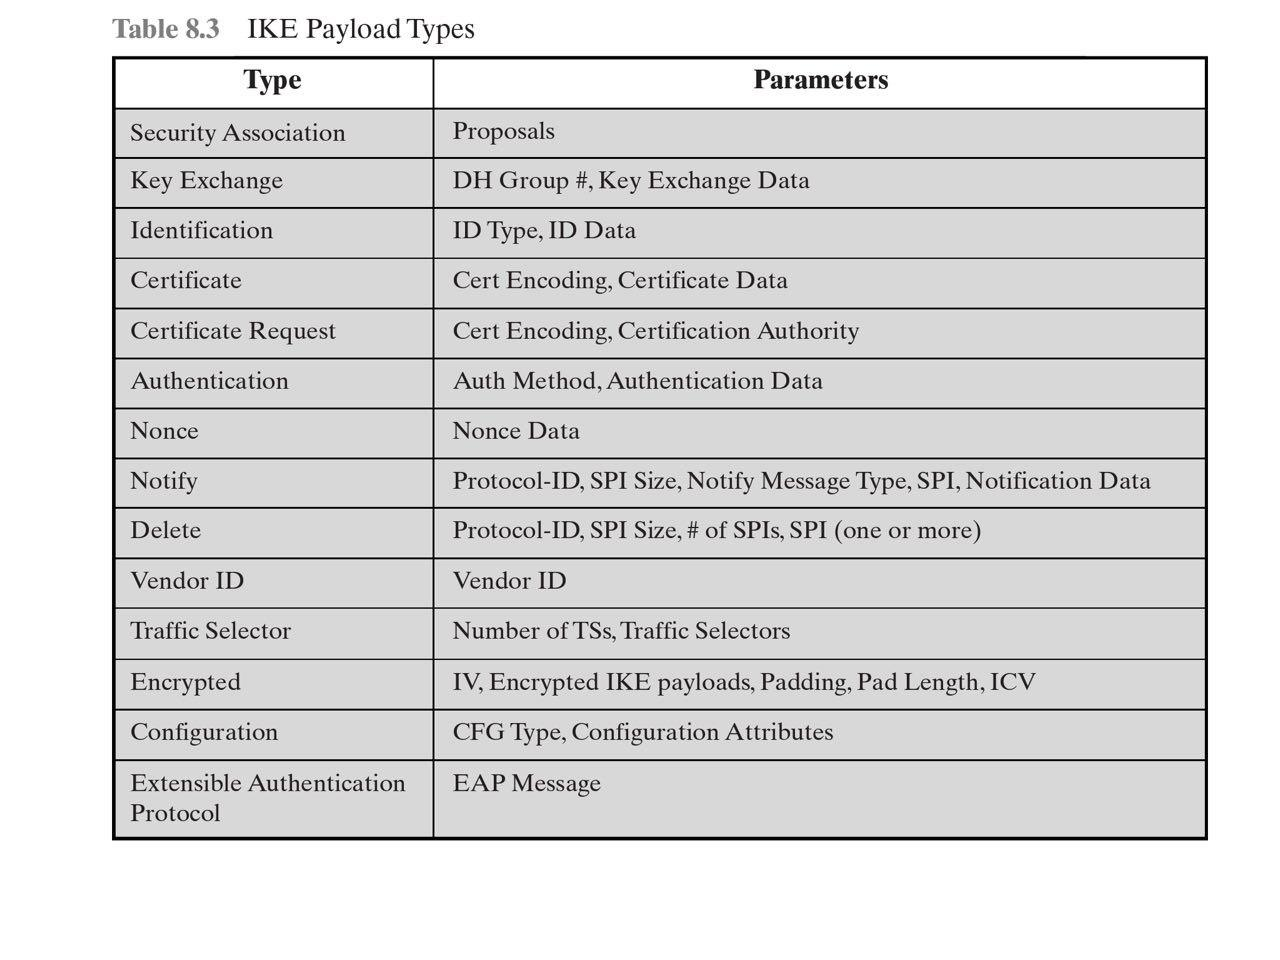
\includegraphics[scale=0.20]{PayloadTypes.jpg}
  \end{center}
}

\frame{\frametitle{Tipos de carga útil de IKE}
  \begin{itemize}
  \item \textbf{Intercambio de llaves (Key exchange payload)}: Especifica la técnica de intercambio de llaves (Oakleay, Diffie-Hellman, PGP).
  \item \textbf{Certificado (Certificate payload)}: Transfiere un certificado de llave pública.
  \item \textbf{Autenticación (Authentication)}: Datos usados para autenticación de mensajes.
  \end{itemize}

}

\frame{\frametitle{Tipos de carga útil de IKE}
  \begin{itemize}
  \item \textbf{Nonce}: Datos aleatorios usados para proteger contra ataques de repetición.
  \item \textbf{Notificación (Notify)}: Contiene errores o información del estado asociado con la SA.
  \item \textbf{Eliminar (Delete)}: Indica uno o mas SAs que el emisor ha eliminado de su base de datos.
  \item \textbf{ID del vendedor (Vendor ID)}: Constante definida por el vendedor que éstos usan para identificar instancias remotas de sus implementaciones.
  \end{itemize}
}

\frame{\frametitle{Tipos de carga útil de IKE}
  \begin{itemize}
  \item \textbf{Selector de tráfico (Traffic Selector)}: Permite a los pares (peers) identificar flujos de paquetes para ser procesados por servicios IPsec.
  \item \textbf{Cifrado (Encrypted)}: Contiene otras cargas útiles cifradas. El formato de esta carga útil es similar el de ESP, puede contener un IV o un ICV.
  \item \textbf{Configuración (Configuration)}: Se usa para intercambiar informacion de las cofiguraciones entre usuarios.
  \item \textbf{Protocolo de autenticación extensible (Extensible Authentication Protocol EAP)}: Permite autenticar SAs de IKE usando EAP.
  \end{itemize}
}

\section{Suites criptográficas}

\frame{\frametitle{Suites criptográficas}
  Tanto \textbf{IPsec} como \textit{IKE}, ambos en sus versión 3, dependen de una gran variedad de
  tipos de algoritmos criptográficos.\\
  \vspace{0.3cm}
  Dos \textbf{RFCs} (\textit{Request for comments}), definen suites de algoritmos criptográficos recomendados y
  parámetros respectivos para diversas aplicaciones.
}

\subsection{RFC 4308}
\frame{\frametitle{RFC 4308}
  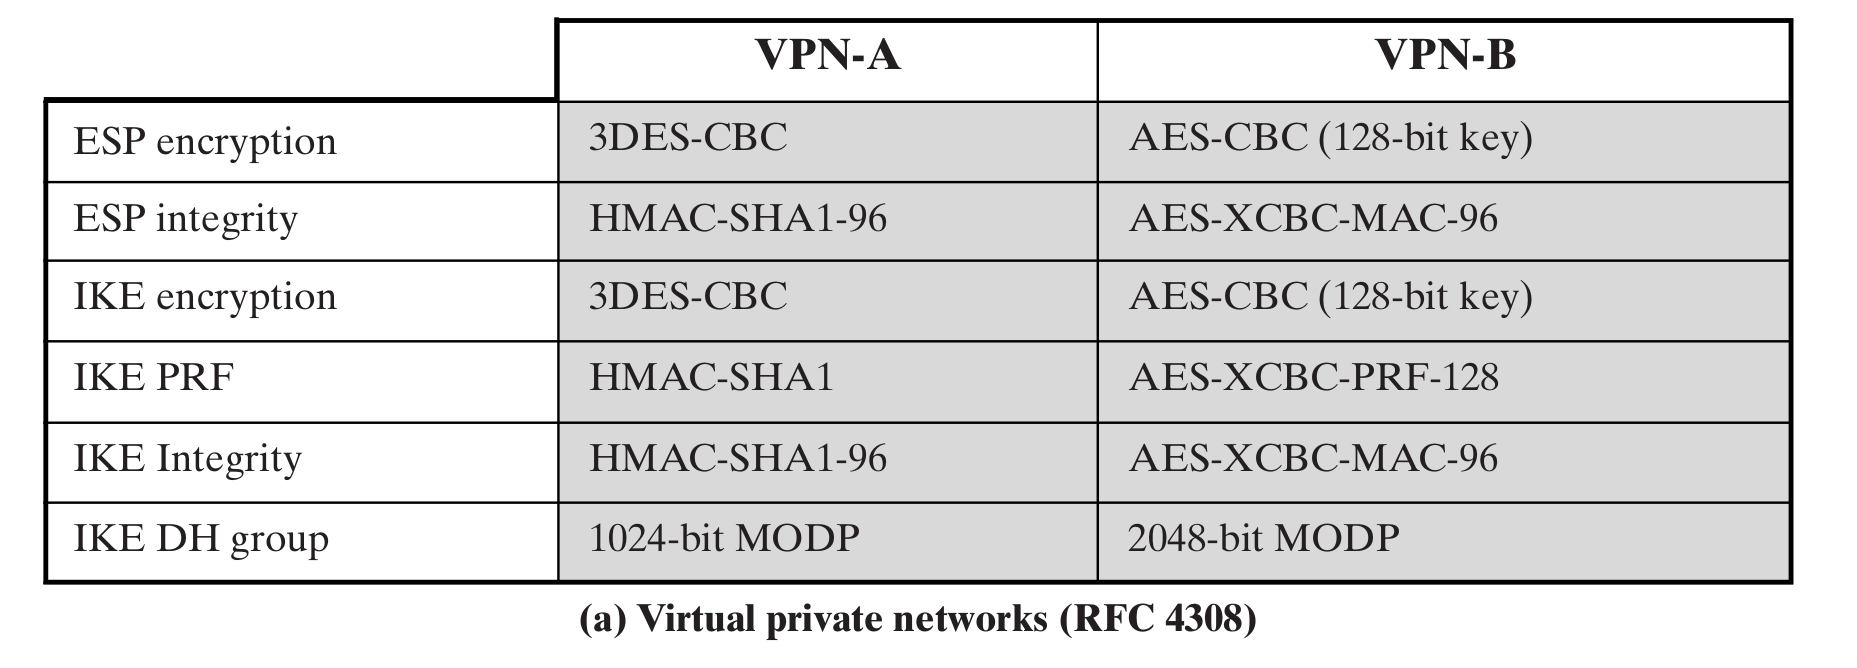
\includegraphics[scale=0.18]{RFC1} 
}

\frame{\frametitle{RFC 4308}
  \begin{itemize}
  \item \textbf{Cifrado:} Cifrado de bloque con modo \textit{CBC}.
  \item \textbf{Autenticación de mensajes:} \textit{VPN-A} $\to$ \textit{SHA-1} o \textit{HMAC} (96 \textit{bits}).
  \item \textbf{Función pseudoaleatoria:} \textit{IKEv2} genera \textit{bits} pseudoaleatorios, a partir del uso del \textit{MAC}, utilizado en la autenticación del mensaje.
  \end{itemize}
}

\subsection{RFC 4869}
\frame{\frametitle{RFC 4869}
  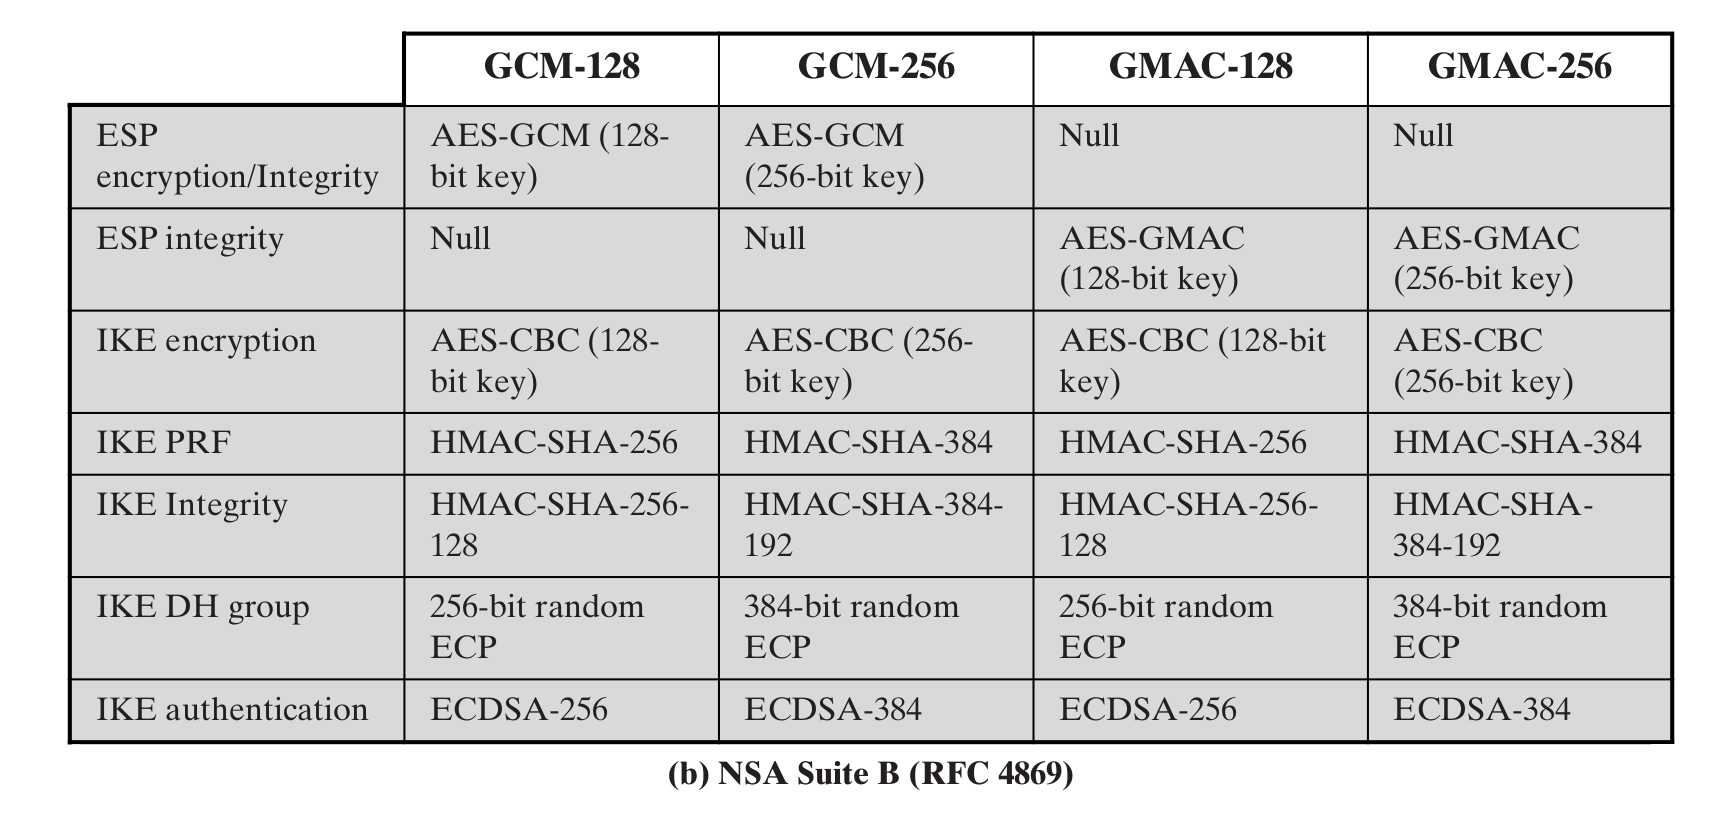
\includegraphics[scale=0.19]{RFC2}
}

\frame{\frametitle{RFC 4869}
  \begin{itemize}
  \item \textbf{Cifrado:} Para \textit{ESP}, cifrado con autenticación se provee utilizando el modo
    GCM con llaves de tamaño 128 o 256 \textit{bits}. Mientras que para cifrado en \textit{IKE}, se utiliza el modo \textit{CBC}.
  \item \textbf{Autenticación de mensajes:} Para \textit{ESP}, si sólo se requiere autenticación, se utiliza el modo GMAC. Mientras que para \textit{IKE}, se provee mediante \textit{HMAC}, con \textit{SHA-3}.
  \item \textbf{Función pseudoaleatoria:} \textit{IKEv2} genera \textit{bits} pseudoaleatorios, a partir del uso del \textit{MAC}, utilizado en la autenticación del mensaje.
  \end{itemize}
}
\end{document}

